\documentclass[pdflatex,sn-mathphys-num,iicol]{sn-jnl}
\usepackage{graphicx,amsmath,amssymb,booktabs,multirow,tabularx}
\usepackage{algorithm,algpseudocode}
\usepackage{xcolor}
\usepackage{microtype}
\hypersetup{pdftitle={Evidence-Linked Multi-Fault Network Troubleshooting with Local Language Models and Twin-Verified Repair},pdfauthor={Muhammad Umair Ahmad},pdfkeywords={network troubleshooting, multi-fault diagnosis, digital twin, local language models}}
\raggedbottom
\setcounter{dbltopnumber}{3}
\renewcommand{\dbltopfraction}{0.9}
\renewcommand{\textfraction}{0.08}
\newcommand{\full}{\textsc{Full}}
\newcommand{\code}[1]{\texttt{\detokenize{#1}}}
\begin{document}
\title[Evidence-linked network troubleshooting]{Evidence-Linked Multi-Fault Network Troubleshooting with Local Language Models and Twin-Verified Repair}
\author*{\fnm{Muhammad Umair} \sur{Ahmad}}\email{i242545@isb.nu.edu.pk}
\affil{\orgname{24i-2545, Section AI-C}}
\abstract{Network troubleshooting requires finding every fault and checking recovery against intended state. A correct diagnosis alone does not establish recovery. This study implements a hybrid workflow for static IPv4 networks with five logical roles, verified incident retrieval, configuration checks, dependency-aware repairs, and twin verification with rollback. The four-device emulated dataset has separate training, development, and evaluation incidents, including healthy, single-fault, and concurrent-fault cases. The evaluation uses three local language models, 294 matched comparative runs, 72 robustness runs, and a separate 21-run evaluation of the revised system. The full workflow achieves 100\% fault-set F1 and exact diagnosis in the comparative study. It matches the rule-based reference and exceeds the best single-agent result by 92.4 percentage points in F1. Without curated incidents, exact diagnosis falls by 7.1--57.1 percentage points across the models. After changes to dependency planning and approval, the revised system achieves 21/21 exact diagnoses and 18/18 verified repairs. Eight controlled safety executions show the expected blocking or rollback behaviour. The results support the tested workflow, with diagnosis, recovery, and component contribution measured separately.}
\keywords{network troubleshooting, multi-fault diagnosis, local language models, retrieval-augmented generation, digital twin, verified remediation}
\maketitle

\section{Introduction}\label{sec:intro}
A network complaint describes a symptom and may not identify its cause. A failed connection can involve a down interface, missing address, incorrect route, or filtering rule. Concurrent faults can also hide one another. Diagnosis and repair therefore require measured network evidence.

Recent studies use structured language-model agents for network troubleshooting. SADE confirms symptoms before escalating the diagnosis \cite{sade}. FaulT-Bench tests unreliable ticket wording and cases where the network is healthy \cite{faultbench}. HANA uses specialized agents for recovery in a 5G core \cite{hana}. These approaches show why the agent needs measured evidence, a clear stopping condition, and separate diagnosis and recovery results.

The research gap concerns how complete multi-fault diagnosis leads to verified recovery in a local network. A correct fault label is not enough if the repair misses a dependency, uses unresolved evidence, or introduces another fault. This study examines configuration checks, verified training incidents, and twin-tested repair using small local models.

Five logical roles share the same local backbone. A trusted controller provides typed measurements and hides injected labels. Repairs follow public intent and measured findings. The main network is changed after the repair succeeds on an equivalent faulty twin.

The contributions are:
\begin{itemize}
\item A working hybrid system that connects the complete fault set to measured evidence, dependency-aware actions, twin verification, and checked rollback.
\item An evaluation across three local backbones using matched baselines, component ablations, perturbed inputs, and separate diagnosis and repair measurements.
\item An analysis of verified incident retrieval and repair-stage changes, supported by a recorded concurrent-fault case and controlled safety executions.
\end{itemize}
The contribution is the complete evidence-to-recovery workflow built on existing multi-fault infrastructure and role-based agents. The remaining sections cover related work, methodology, experimental setup, results, base-paper comparison, ablation, discussion, and conclusion.

\section{Related work / literature review}\label{sec:related}
\subsection{Structured diagnosis and evidence collection}
SADE starts with an initial scan, performs a deeper scan when needed, identifies the fault family, and applies the relevant skills. Its published evaluation reports RCA F1 of 0.77 and detection accuracy of 0.85 on matched NIKA cases \cite{sade}. This study adapts its pinned skills as a local baseline and adds intent-state confirmation and verified repair. Scores apply to the adaptation, which uses different models and tools.

NIKA provides a reproducible incident framework and an extensible interface between the agent and the network \cite{nika,playground}. It covers 54 network issues across multiple scenarios and supports controlled, coordinated fault injection. This study follows that incident design. Its reported agent scores come from the local four-device network.

\subsection{Knowledge-supported and hybrid approaches}
NetSemantic converts network information into semantic and symbolic representations, then retrieves a knowledge graph for diagnosis. It reports 89.49\% fault-diagnosis accuracy \cite{netsemantic}. Hy-LIFT combines rules, semi-supervised classification, and LLM explanations on operator logs, with macro-F1 of 0.89 \cite{hylift}. Both studies support structured or hybrid diagnosis. This work also evaluates concurrent fault sets and checks configuration recovery after executing the repair.

The knowledge base in this study contains frozen documentation and verified training incidents. The documentation-only ablation measures the effect of removing those incidents. Evaluation cases do not enter memory.

\subsection{Operational autonomy and reliable evaluation}
HANA uses a hierarchical architecture and shared memory to coordinate executive agents. In its 5G-core case studies, repair time for an unreachable AMF node falls from 36 to 5 minutes \cite{hana}. That experiment measures operational recovery in a different domain. This study instead tests complete local configuration diagnosis and repairs on a twin that reproduces the faulty state.

FaulT-Bench evaluates 200 core scenarios across eight topologies using accurate and misleading tickets. Its outcome score falls from 0.932 on correct-fault tickets to 0.820 on false-premise tickets \cite{faultbench}. These scores come from a judge and differ from set-level F1. This study therefore includes a healthy case and perturbed tickets, while checking the diagnosis directly against injected faults. Table~\ref{tab:literature} summarizes the base papers and related studies.

\begin{table*}[t]
\caption{Base papers and related studies. Asterisks mark results reported by the original authors. Different datasets, metrics, and settings prevent a direct ranking.}\label{tab:literature}
\centering\scriptsize
\begin{tabularx}{\textwidth}{@{}>{\raggedright\arraybackslash}p{1.65cm}>{\raggedright\arraybackslash}p{1.7cm}>{\raggedright\arraybackslash}p{2.25cm}>{\raggedright\arraybackslash}p{2.2cm}>{\raggedright\arraybackslash}p{2.0cm}>{\raggedright\arraybackslash}X@{}}
\toprule
Study & Problem & Method & Dataset / setting & Metric and result* & Comparison boundary / remaining need \\
\midrule
Tseng et al., 2026 \cite{sade} & Root-cause diagnosis & Symptom escalation and skill library & 523 matched NIKA test cases; Claude Sonnet 4.6 & RCA F1 0.77; detection 0.85 & Manually maintained skills; local adaptation differs in tools and backbone. \\
Tseng et al., 2026 \cite{faultbench} & Unreliable tickets & SADE, ReAct, Claude Code; LLM judging & 200 core cases; eight topologies & Outcome 0.932 correct-fault; 0.820 false-premise & Judge-based outcome and healthy-network stopping; not executed repair success. \\
Wu et al., 2026 \cite{hana} & 5G autonomy & Hierarchical orchestrator, memory, executive agents & 5G-core case studies & AMF repair: 36 to 5 min; 86.11\% reduction & Different domain and MTTR setting; no matched local fault-set score. \\
Tan et al., 2025 \cite{netsemantic} & Multimodal diagnosis & Semantic and symbolic conversion and knowledge graph & NS-3 network scenarios & Diagnosis accuracy 89.49\% & Diagnosis reports; executed twin-tested recovery is a separate task. \\
Salman et al., 2025 \cite{hylift} & Log diagnosis & Rules, semi-supervised classifier, LLM & 8,000 operator-log sequences & Macro-F1 0.89 & Private log setting and class labels differ from concurrent configuration faults. \\
\bottomrule
\end{tabularx}
\end{table*}

\section{Proposed methodology}\label{sec:method}
\subsection{Problem formulation and objective}
Let $G=(V,E)$ denote the network topology, where $V$ is the set of devices and $E$ contains their links and configuration dependencies. Let $I$ be the public intended state, $t$ the ticket, and $O$ the measured observations. The hidden injected fault set is $F$. Each fault is written as $(d,f,u)$, with device $d$, fault family $f$, and target $u$. The system returns the estimated fault set $\widehat F$ and an ordered repair plan $A$. Every finding must refer to an observation identifier in $O$.

The objective is to restore the network within the tool, token, and time budgets. Model parameters are fixed, so there is no task-specific training loss. Repair selection follows the constrained objective below:
\begin{equation}
\min_A |A| \quad \text{subject to}\quad
\begin{cases}
A\subseteq\mathcal{A}(I,O,\widehat F),\\
\operatorname{complete}(A)=1,\\
\operatorname{policy}(A)=1,\\
\operatorname{ok}(S_{\mathrm{twin}},A,I)=1.
\end{cases}\label{eq:objective}
\end{equation}
Here $|A|$ is the number of actions, $\mathcal{A}$ is the set of permitted restorative templates, and $\operatorname{ok}$ checks recovery from twin state $S_{\mathrm{twin}}$. The system enforces Equation~\ref{eq:objective} through complete action templates and dependency order.

\subsection{Architecture and information boundaries}
Figure~\ref{fig:architecture} shows the system architecture. The orchestrator maintains the hypotheses and execution budget. The diagnostic role proposes faults and cites their evidence. The knowledge role retrieves relevant passages. The remediation role prepares typed actions with preconditions, expected effects, post-checks, and rollback instructions. Oversight records the model review and applies the approval checks.

The roles share the selected backbone; the controller handles deployment, measurement, and execution. An unprivileged, read-only agent container cannot access the Docker socket, private labels, or injection code. Its broker accepts interface, address, route, firewall, and fixed-target ping queries, rejecting arbitrary shell commands and out-of-lab targets.

\begin{figure*}[t]
\centering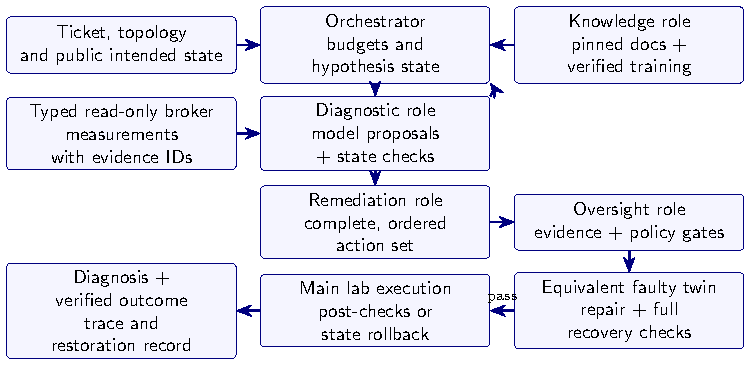
\includegraphics[width=0.84\textwidth]{figures/architecture.pdf}
\caption{Evidence-linked troubleshooting architecture. Solid arrows show the main workflow; the dashed arrow shows additional measurements. The knowledge snapshot remains frozen during evaluation.}\label{fig:architecture}
\end{figure*}

\subsection{Evidence confirmation and concurrent faults}
The system first reads interface state, IPv4 addresses, routes, and filtering rules from every device, then runs end-to-end probes. Each measurement retains its raw output, timestamp, device, origin, and evidence identifier. The hybrid variants compare public intended state with these measurements to confirm the fault set. They reject unsupported model proposals and retain directly measured faults even when the model misses them. The evaluation also tests these configuration checks as a rule-based reference.

The topology dependencies help distinguish a root cause from its consequences. A down interface or missing address can also remove a gateway route. The absent route remains consequence evidence unless it independently contradicts routing intent after the dependency is considered. The original workflow uses up to three diagnostic passes to check remaining symptoms. The revised workflow uses one model diagnosis pass, targeted confirmation, and post-repair residual checks. It retries unavailable measurements once within the tool budget. If the evidence remains unresolved, automatic repair approval is blocked.

\subsection{Verified incident retrieval}
The documentation covers Linux forwarding, interface and route operations, filtering, and FRR static routing \cite{kernel,iproute,iptables}. HTML text is normalized into 240-word windows with a 180-word stride. BM25 uses $k_1=1.5$ and $b=0.75$. The local \code{all-minilm:latest} model produces the dense vectors. For passage $p$, the system combines lexical and dense ranks as follows:
\begin{equation}
\operatorname{RRF}(p)=\frac{1}{60+r_{\mathrm{lex}}(p)}+
\frac{1}{60+r_{\mathrm{dense}}(p)},\label{eq:rrf}
\end{equation}
where ranks start at one. Each retriever supplies its top 20 passages. The best six fused candidates are reranked locally, and four passages are returned.

A training incident is accepted into memory only after completed execution, exact diagnosis, valid evidence references, twin equivalence, successful recovery, regression checks, and final restoration. This is semi-automatic curation of verified incidents; unrestricted continual learning was not evaluated. Frozen snapshots retain document hashes, vectors, embedding identity, and incident provenance.

\subsection{Dependency-aware repair and verification}
The permitted operations restore a link, address, route, or filtering state to public intent. Actions contain typed fields instead of generated shell text. A dependent repair may include a missing default or static route when measured absence, intended subnet relationships, and the matching link or address repair justify it. Links are restored before addresses, routes, and filters.

The revised planner must return the complete set of distinct actions. Duplicates, omissions, unrelated changes, and unsupported actions are rejected. The controller then checks policy and fresh fault preconditions. The twin must match the captured faulty configuration and connectivity. Recovery requires intended state and six scored connectivity paths; bounded convergence warmups are recorded separately. The snapshot contains administrative interface state, IPv4 addresses, gateway routes, and the complete normalized IPv4 filter table. Docker NAT/DNS bookkeeping is outside this incident snapshot. If main-network execution or post-checks fail, the controller restores the pre-repair state and checks restoration fidelity.

The Phase 2 proposal changed during implementation. Model review initially vetoed repairs; the revised full workflow records it as advice. Approval requires measured evidence, complete actions, and no unresolved findings. Twin, policy, precondition, and post-repair checks remain mandatory. Changes follow development and original-study evidence; no separate instructor-feedback record was available. Algorithm~\ref{alg:workflow} describes the revised full workflow.

\begin{algorithm}[t]
\caption{Revised evidence-linked diagnosis and repair}\label{alg:workflow}
\begin{algorithmic}[1]
\Require Ticket $t$, topology $G$, public intent $I$, frozen memory $K$
\State Capture the faulty main-network state $S_0$
\State $O\gets$ typed measurements; retry unavailable data once
\State Retrieve passages from $K$ using $t$, $G$, and symptom context
\State Obtain model hypotheses and confirm $\widehat F$ against $(I,O)$
\State Record diagnosis before entering the repair stage
\If{healthy, unresolved evidence, or exhausted budget}
\State \Return diagnosis and recorded stopping reason
\EndIf
\State Generate complete distinct restorative actions $A$
\State Check evidence, action completeness, policy, and fresh preconditions
\If{any approval check fails} \State \Return blocked repair \EndIf
\State Restore twin to $S_0$ and verify equivalence
\State Execute $A$ on twin in dependency order
\If{twin recovery fails} \State \Return blocked repair \EndIf
\State Execute $A$ on main network and check state and connectivity
\If{execution or post-checks fail}
\State Restore $S_0$ and verify rollback fidelity
\EndIf
\State \Return diagnosis, repair outcome, and trace
\end{algorithmic}
\end{algorithm}

\section{Experimental setup}\label{sec:setup}
\subsection{Dataset and preprocessing}
The evaluated network is the four-device chain $\mathrm{pc1}\! -\!\mathrm{r1}\! -\!\mathrm{r2}\! -\!\mathrm{pc2}$ with static IPv4 routes and filtering rules. It runs real network processes in Docker/Kathar\'{a} emulation \cite{kathara,docker}. The subnets are 10.0.1.0/24, 10.0.12.0/30, and 10.0.2.0/24. Standard evaluation cases include a healthy network, individual link, route, address, and filter faults, and two- and three-fault combinations. Table~\ref{tab:data} gives the split and run design. The verified injected fault set is the ground truth and remains hidden from the agent.

\begin{table}[t]
\caption{Local dataset splits and evaluated execution blocks. Runs are model-case executions, not independent incidents.}\label{tab:data}
\centering\small
\begin{tabular}{@{}p{2.45cm}p{4.45cm}@{}}
\toprule
Split / block & Size and purpose \\
\midrule
Training & 3 incidents for verified memory \\
Development & 3 incidents for workflow investigation \\
Evaluation & 7 standard incidents; ticket variants remain in their incident split \\
Comparative & $7$ methods $\times7$ cases $\times3$ models $\times2$ repeats $=294$ runs \\
Robustness & $3$ incidents $\times2$ conditions $\times2$ methods $\times3$ models $\times2$ repeats $=72$ runs \\
Revised follow-up & $7$ cases $\times3$ models $\times1$ repeat $=21$ runs \\
\bottomrule
\end{tabular}
\end{table}
Tickets and observations are normalized into structured records. A failed measurement is kept as unavailable, not treated as proof of a missing configuration. Ticket variants stay with their source incident, and only training incidents enter accepted memory. Related cases remain in three incident groups for statistical analysis. The local scores do not include the full NIKA and FaulT-Bench corpora.

\subsection{Baselines and ablations}
The original study compares seven methods using the same model, case, seed, and budget conditions. \code{rule_based} checks measured state against intent and uses the shared constrained model planner for repairs. \code{single_agent} uses tools and retrieval without full hybrid confirmation. \code{sade_local} adapts the pinned SADE skill library and escalation procedure \cite{saderepo} to the local tools and performs diagnosis only. The remaining methods are \code{full} and its \code{no_curation}, \code{no_rescan}, and \code{no_twin} ablations.

No-curation removes accepted incidents from retrieval. No-rescan retains the initially supported findings and removes further scanning. No-twin retains the other execution controls. Phase 2 also proposed plain-LLM, RAG-only, and additional role and policy ablations. These options exist in the implementation but were not part of the completed comparison matrix, so they are not reported as evaluated baselines.

\subsection{Implementation and reproducibility}
The three backbones are \code{llama3.2:1b}, \code{qwen2.5-coder:3b}, and \code{qwen2.5:1.5b}, served locally through Ollama \cite{ollama}. The recorded host is macOS ARM64 with 8 GiB RAM. Models are loaded one at a time. Llama uses Q8\_0 quantization, and both Qwen models use Q4\_K\_M. The environment records Python 3.12.16, Pydantic 2.14.3, NumPy 2.5.4, SciPy 1.18.1, and requests 2.34.2. The dependency lock preserves these experiment versions.

The original protocol uses seeds 1000 and 1001, temperature 0.2, a 1,024-token output cap, an 8,192-token inference context, a 24,000-token investigation budget, a 240-second investigation budget, and 48 tool calls. Setup, repair, and verification can add to total runtime and token use. The revised protocol uses seed 1000 and temperature zero with the same investigation limits. Seed requests are logged, although outputs may differ across runtime environments. Local inference has zero API charges. Energy and hardware costs were not measured.

The submission includes code, labs, source archives, raw records, locks, and knowledge snapshots. Replay uses the corresponding study archive. Original and revised code/source hashes begin \code{e1140771a2a1} and \code{cad5d3c7f004}, respectively. The reproduction guide gives entry points. Per-run model and image digests avoid mutable tags.

\subsection{Metrics and statistical analysis}
For a faulty case, precision $P$, recall $R$, and F1 are
\begin{equation}
P=\frac{|\widehat F\cap F|}{|\widehat F|},\quad
R=\frac{|\widehat F\cap F|}{|F|},\quad
F_1=\frac{2PR}{P+R}.\label{eq:metrics}
\end{equation}
A faulty case with a zero denominator scores zero. Exact match is $\mathbb{1}[\widehat F=F]$. When $F=\varnothing$, the system must explicitly report a healthy network. Comparative mean F1 uses faulty cases, while exact match includes healthy cases. Repair success is verified recovery divided by all faulty executions, including blocked and failed attempts. SADE-local has no repair score.

Paired differences are averaged within incident groups. The saved analysis uses 2,000 group-bootstrap draws, seed 42, 95\% percentile intervals, and paired Wilcoxon tests with Holm adjustment. Repeated executions are not independent incidents. Model-output and budget failures remain in the results. Infrastructure retries keep the same configuration and seed, and the earliest restored outcome is selected. Diagnosis is saved before remediation so a later failure does not erase a completed diagnosis.

\section{Results and analysis}\label{sec:results}
\subsection{Matched comparative evaluation}
Table~\ref{tab:core} reports every model-method condition in the 294-run comparative study. The full workflow achieves 100\% mean fault-set F1 and exact diagnosis across 42 standard executions. The rule-based reference also reaches 100\%. Equal scores show the contribution of configuration checks alongside model reasoning.

\begin{table*}[t]
\caption{Original matched study: 14 standard executions per model-method condition. F1 averages faulty cases; exact match includes the healthy case. Repair uses all 12 faulty executions per condition. Tokens are mean recorded total tokens, rounded to the nearest integer.}\label{tab:core}
\centering\small
\begin{tabular}{@{}llrrrrr@{}}
\toprule
Backbone & Method & F1 (\%) & Exact (\%) & Repair (\%) & Mean time (s) & Mean tokens \\
\midrule
\multirow{7}{*}{Llama 3.2 1B} & Full & 100.0 & 100.0 & 0.0 & 49.6 & 19,366 \\
 & Rule-based & 100.0 & 100.0 & 8.3 & 167.5 & 780 \\
 & Single agent & 0.0 & 0.0 & 0.0 & 45.6 & 16,948 \\
 & SADE-local & 0.0 & 0.0 & N/A & 54.3 & 18,002 \\
 & No curation & 91.7 & 92.9 & 0.0 & 57.7 & 19,740 \\
 & No rescanning & 100.0 & 100.0 & 0.0 & 42.9 & 13,420 \\
 & No twin & 100.0 & 100.0 & 0.0 & 48.6 & 19,947 \\
\midrule
\multirow{7}{*}{Qwen 2.5 Coder 3B} & Full & 100.0 & 100.0 & 8.3 & 141.8 & 22,480 \\
 & Rule-based & 100.0 & 100.0 & 16.7 & 172.7 & 806 \\
 & Single agent & 7.6 & 0.0 & 0.0 & 97.6 & 19,401 \\
 & SADE-local & 3.9 & 0.0 & N/A & 73.9 & 16,352 \\
 & No curation & 85.2 & 85.7 & 0.0 & 98.2 & 20,942 \\
 & No rescanning & 100.0 & 100.0 & 0.0 & 80.2 & 14,485 \\
 & No twin & 79.2 & 78.6 & 8.3 & 110.4 & 21,717 \\
\midrule
\multirow{7}{*}{Qwen 2.5 1.5B} & Full & 100.0 & 100.0 & 16.7 & 124.2 & 24,702 \\
 & Rule-based & 100.0 & 100.0 & 50.0 & 123.6 & 775 \\
 & Single agent & 2.4 & 0.0 & 0.0 & 62.5 & 19,573 \\
 & SADE-local & 3.7 & 0.0 & N/A & 68.9 & 18,623 \\
 & No curation & 41.7 & 42.9 & 0.0 & 65.1 & 12,379 \\
 & No rescanning & 100.0 & 100.0 & 16.7 & 104.3 & 15,193 \\
 & No twin & 100.0 & 100.0 & 75.0 & 107.1 & 35,304 \\
\bottomrule
\end{tabular}
\end{table*}
For Qwen Coder, single-agent F1 is 7.6\% and SADE-local is 3.9\%. These results include model and budget failures.

The original full pipeline diagnoses the standard cases correctly but verifies repair in only 3/36 faulty executions. Other configurations repair more cases: Qwen 1.5B without the twin reaches 75.0\%, and its rule-based condition reaches 50.0\%. The records identify repair omissions, dependency handling, and model vetoes as issues. Section~\ref{sec:method} describes the resulting changes. Figure~\ref{fig:performance} shows diagnosis, recovery, time, and robustness together, since a correct diagnosis alone does not show that repair succeeded.

\begin{figure*}[t]
\centering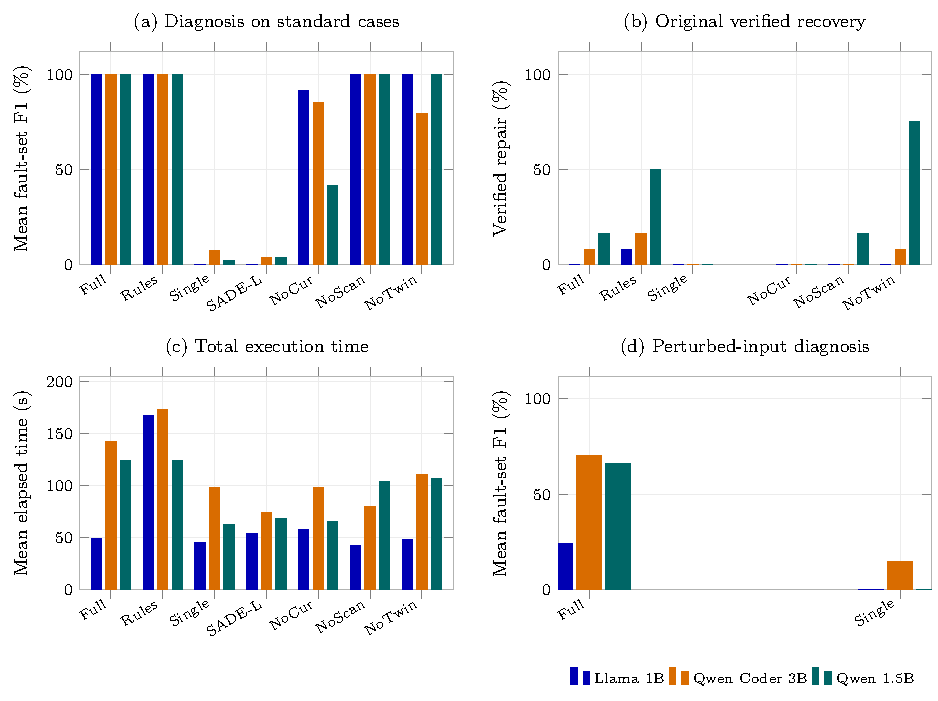
\includegraphics[width=0.94\textwidth]{figures/performance.pdf}
\caption{Original-study measurements from the saved Phase 3 records. Panels (a)--(c) use standard cases; panel (d) uses the 72-run perturbed-input block. Each colour is a local backbone. SADE-L is the local adaptation; its repair score is not applicable and is omitted. NoCur, NoScan, and NoTwin denote the three component removals.}\label{fig:performance}
\end{figure*}

\subsection{Revised end-to-end evaluation}
Table~\ref{tab:revised} gives the separate revised-system results. Each backbone exactly diagnoses all seven cases and verifies repair on all six faulty cases. The total is 21/21 exact diagnoses and 18/18 verified repairs. The healthy case requires no repair. These results evaluate the revised planning and approval workflow together.

\begin{table}[t]
\caption{Revised full-system follow-up. Each model has one execution of each standard case. Runtime includes setup and verification.}\label{tab:revised}
\centering\small
\begin{tabular}{@{}lrrr@{}}
\toprule
Backbone & Exact & Repair & Mean s \\
\midrule
Llama 3.2 1B & 7/7 & 6/6 & 111.7 \\
Qwen Coder 3B & 7/7 & 6/6 & 167.3 \\
Qwen 2.5 1.5B & 7/7 & 6/6 & 113.2 \\
\midrule
Total & 21/21 & 18/18 & -- \\
\bottomrule
\end{tabular}
\end{table}
The revised study was run after examining the earlier results and changes both temperature and workflow. The change from 3/36 to 18/18 repairs describes the development outcome. Matched baseline and ablation comparisons still use the original study.

\subsection{Statistical evidence and execution cost}
Table~\ref{tab:stats} gives selected saved group-level intervals for Qwen 1.5B. The mean full-minus-single-agent difference is 0.990, with a bootstrap interval of [0.971, 1.000]. Against SADE-local, the difference is 0.985, with [0.956, 1.000]. Group weighting accounts for the small differences from Table~\ref{tab:core}. All saved Holm-adjusted $p$-values are 1.000. With three incident groups, these results do not support a confirmatory significance claim.

\begin{table}[t]
\caption{Exploratory group-level F1 differences for Qwen 1.5B, full minus comparator. Intervals and tests use three incident groups.}\label{tab:stats}
\centering\small
\begin{tabular}{@{}lrrr@{}}
\toprule
Comparator & Mean $\Delta$ & 95\% interval & Raw $p$ \\
\midrule
Single agent & 0.990 & [0.971, 1.000] & 0.25 \\
SADE-local & 0.985 & [0.956, 1.000] & 0.25 \\
No curation & 0.533 & [0.500, 0.600] & 0.25 \\
Rule-based & 0.000 & [0.000, 0.000] & 1.00 \\
\bottomrule
\end{tabular}
\end{table}
The original full workflow takes a mean of 49.6, 141.8, and 124.2 seconds for Llama, Qwen Coder, and Qwen 1.5B. A blocked repair can finish early, so runtime should be considered with the recovery result. Rule-based token totals also include the shared model repair planner.

\subsection{Robustness and qualitative evidence}
The robustness tests use misleading tickets and unavailable route telemetry. Full-workflow F1 is 24.4\% for Llama, 70.3\% for Qwen Coder, and 66.1\% for Qwen 1.5B. The corresponding single-agent scores are 0.0\%, 14.6\%, and 0.0\%. Exact diagnosis is 0.0\%, 41.7\%, and 41.7\% for the full workflow and zero for every single-agent condition. The full system performs better, although partial findings can still miss the complete fault set. If measurements remain unavailable, the system retains that uncertainty and the revised full workflow blocks repair approval.

Figure~\ref{fig:case} shows a revised Qwen 1.5B triple-fault run. The system identifies the missing pc2 address, down r2 interface, and absent r2 route. It also restores pc2's default route as a repair dependency. Measured state and intent justify that action, but it is not another injected root cause. Twin verification and post-repair checks both pass. The case therefore has more repair actions than root causes.

\begin{figure*}[t]
\centering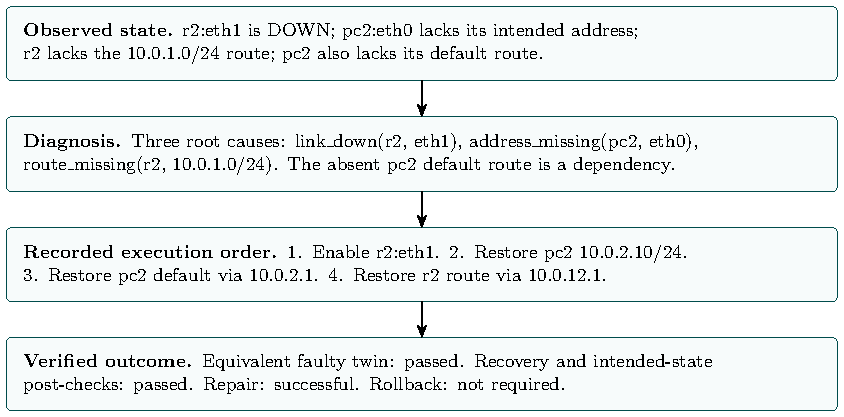
\includegraphics[width=0.86\textwidth]{figures/case-trace.pdf}
\caption{Recorded qualitative example: the revised Qwen 1.5B triple-fault run. Three root causes require four ordered actions because address restoration also requires restoring the dependent default route. Source record: \code{849e2a1ec38c0a8d404d0a52.json}.}\label{fig:case}
\end{figure*}

\section{Comparison with base papers and state of the art}\label{sec:comparison}
\subsection{Fair quantitative comparison}
Table~\ref{tab:literature} keeps the original metric names and settings. SADE's RCA F1 of 0.77 cannot be compared directly with local F1 because the backbone, topology, tools, and scoring differ. HANA and FaulT-Bench also have no matched local measurements. Absolute and relative gains over their published scores cannot therefore be calculated fairly.

The matched comparison uses SADE-local and the other local methods in Table~\ref{tab:core}. Table~\ref{tab:gains} reports the full workflow's F1 improvement from unrounded means. Absolute gain is $100(F_{1,\mathrm{full}}-F_{1,b})$ percentage points. Relative gain is $100(F_{1,\mathrm{full}}-F_{1,b})/F_{1,b}$ percent for baseline $b$. Relative gain is undefined for a zero baseline. Full and rule-based diagnosis have equal scores, so the gain is zero for all three models.

\begin{table*}[t]
\caption{Matched local F1 improvement over the single-agent comparator and SADE-local. These are local measurements, not improvements over original published scores. Large relative values reflect small nonzero comparator scores.}\label{tab:gains}
\centering\small
\begin{tabular}{@{}lrrrr@{}}
\toprule
Backbone & Gain over single (pp) & Relative (\%) & Gain over SADE-local (pp) & Relative (\%) \\
\midrule
Llama 3.2 1B & 100.00 & Undefined & 100.00 & Undefined \\
Qwen Coder 3B & 92.43 & 1,221.7 & 96.06 & 2,441.2 \\
Qwen 2.5 1.5B & 97.62 & 4,100.0 & 96.30 & 2,600.0 \\
\bottomrule
\end{tabular}
\end{table*}

\subsection{Methodological differences and source of gain}
Intent-state checks account for complete diagnosis in both the full system and the rule-based reference. Retrieval supplies relevant context. The revised action contract checks that no required repair is omitted, and twin execution and post-checks verify recovery.

HANA evaluates an operational hierarchy, while this study tests a bounded repair contract with explicit twin equivalence. FaulT-Bench focuses on ticket assessment. This work separately records correct diagnosis, blocked plans, and verified recovery. A ranking across these domains would require matched experiments.

\section{Ablation study}\label{sec:ablation}
\subsection{Knowledge, rescanning, and twin removal}
Figure~\ref{fig:ablation} shows how exact diagnosis changes when each tested component is removed. Without curated incidents, exact match falls by 7.1 points for Llama, 14.3 for Qwen Coder, and 57.1 for Qwen 1.5B. Faulty-case F1 falls to 91.7\%, 85.2\%, and 41.7\%, respectively. The curated configuration therefore contributes to the complete workflow. Model termination and later checkpoints also affect the outcome, so this ablation does not show that retrieval alone determines the final rule-confirmed labels.

\begin{figure*}[t]
\centering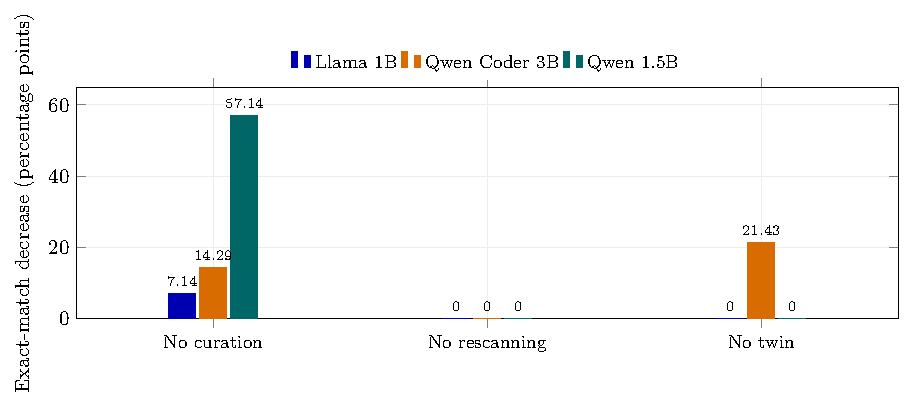
\includegraphics[width=0.84\textwidth]{figures/ablation.pdf}
\caption{Original-study component ablations. Bars give full minus ablation exact match, in percentage points. Zero indicates equal complete-diagnosis rates on the standard cases, not a general claim that the component is unnecessary.}\label{fig:ablation}
\end{figure*}
Without rescanning, standard diagnosis stays unchanged and mean time falls by 6.8, 61.6, and 20.0 seconds for Llama, Qwen Coder, and Qwen 1.5B. The initial sweep already reveals the tested standard faults. Additional passes therefore take time without improving their diagnosis, which supports the targeted revised workflow. The experiment does not establish the same result for faults that become observable only after a repair.

Without the twin, Qwen Coder exact match falls by 21.4 points and the other two models remain unchanged. Qwen 1.5B repair rises from 16.7\% to 75.0\%. Removing the twin from a stochastic pipeline also changes generated plans and their interaction with approval checks. This ablation therefore cannot isolate the twin's safety effect. The controlled tests keep proposal type fixed to examine that effect directly.

\subsection{Controlled safety and isolation checks}
Table~\ref{tab:safety} reports eight controlled executions using four proposal conditions, each tested with and without twin verification. A valid plan recovers the network. An incomplete plan is blocked by twin recovery checks; without the twin, it is executed and then rolled back. Policy blocks unsafe proposals in both settings. Induced post-repair regression also triggers rollback in both. All eight expected-behaviour checks pass. These specified-plan tests are reported separately from agent-generated repair scores.

\begin{table*}[t]
\caption{Controlled safety executions: one execution per row and setting, eight in total. Fundamental containment and policy remain enabled without the twin.}\label{tab:safety}
\centering\small
\begin{tabularx}{\textwidth}{@{}p{3.2cm}XX@{}}
\toprule
Proposal condition & With twin verification & Without twin verification \\
\midrule
Valid repair & Verified successful repair & Verified successful repair \\
Incomplete repair & Blocked before main execution & Main execution followed by rollback \\
Unsafe action & Blocked by policy & Blocked by policy \\
Induced post-repair regression & Rollback after failed post-check & Rollback after failed post-check \\
\bottomrule
\end{tabularx}
\end{table*}
Two additional live checks test agent isolation and real twin recovery/rollback. The isolation record shows UID 65534, no access to the Docker socket, and no access to private fault labels. These checks verify the implemented execution boundary and recovery controls.

\section{Discussion}\label{sec:discussion}
\subsection{Why the workflow works}
The original study achieves complete diagnosis but does not consistently recover the network. The revised system requires every justified action, handles routing dependencies, and approves repairs from measured evidence. With these changes, it verifies 18/18 repairs on the standard cases.

Configuration checks confirm faults. Models propose diagnoses, select knowledge, prepare plans, and review them. Evidence supports findings, findings justify actions, and post-checks verify recovery. Frozen memory and recorded identities allow inspection.

The system can assist troubleshooting where network intent is declared and device access is typed. Supporting another protocol requires corresponding observation and action contracts.

\subsection{Research objectives achieved}
The revised evaluation confirms diagnosis and repair of the tested two- and three-fault sets. The curation ablation measures the contribution of verified incidents, and training-only acceptance provides a reproducible way to update memory. Twin equivalence, post-checks, blocking, and rollback work as designed in the repair tests. All three backbones also have recorded time, tokens, tool calls, and traces. These results address the central Phase 1--2 gap within the implemented static-network setting.

Broader topology coverage, full published-benchmark agent evaluation, independent explanation ratings, and separate oversight and circuit-breaker ablations remain for further study. The completed experiments evaluate the combined workflow and three component removals. They do not measure the separate benefit of every implemented module.

\subsection{Limitations and threats to validity}
The evaluation covers one static IPv4 topology and a defined set of configuration faults. Seven evaluation incidents and three related incident groups limit generalization. The revised follow-up is exploratory because it follows development feedback and changes temperature. Observed failures include small-backbone output errors and unresolved telemetry. SADE-local also differs from the published setting. Further tests should cover dynamic routing and more topologies; the current results establish complete standard-case diagnosis, checked recovery, and the reported component behaviour within this network.

\section{Conclusion and future work}\label{sec:conclusion}
This study implements a network troubleshooting system that uses measured evidence to connect complete diagnosis with dependency-aware, twin-verified repair. In the original comparative study, the full workflow reaches 100\% fault-set F1 and exact diagnosis, equal to the rule-based reference. The curation ablation measures the contribution of verified incident knowledge. In the separate revised evaluation, the system achieves 21/21 exact diagnoses and 18/18 verified repairs across three local models. Controlled tests show the expected policy blocking and rollback behaviour. Future work should extend the measurement and repair contracts to more topologies and dynamic routing, using fresh incidents and matched revised baselines.

\section{Declarations and acknowledgements}\label{sec:declarations}
\textbf{Data and code availability.} The course submission includes the implementation, local cases, private evaluator labels, frozen knowledge snapshots, original and revised source archives, and raw records. The paper package includes audited summary data and vector-figure sources. The code and experimental records are available at \url{https://github.com/Muhammad-Umair-Ahmad/Autonomous-Troubleshooting-Agents}. The reproduction guide gives setup and replay commands.

\textbf{Competing interests.} The author declares no competing interests.

\textbf{Funding.} No external funding is reported for this course project.

\textbf{AI-tool usage.} OpenAI Codex assisted with reviewing the project artifacts, drafting and editing the manuscript, preparing LaTeX and figures, and checking values against saved records. All reported outcomes come from the Phase 3 experiments. The author should review and approve the manuscript before submission.

\textbf{Acknowledgements.} The study uses the open-source NIKA, SADE, FaulT-Bench, Kathar\'{a}, Docker, Ollama, and Linux networking tools cited in this paper.

\bibliography{references}

\end{document}
